\documentclass[../ClassicThesis.tex]{subfiles}
\begin{document}

%************************************************
\chapter{Architecture}\label{ch:architecture}
%************************************************

\newcommand\myNotes[1]{\textcolor{red}{#1}}

\section{Architecture Overview}
%************************************************

\begin{figure}
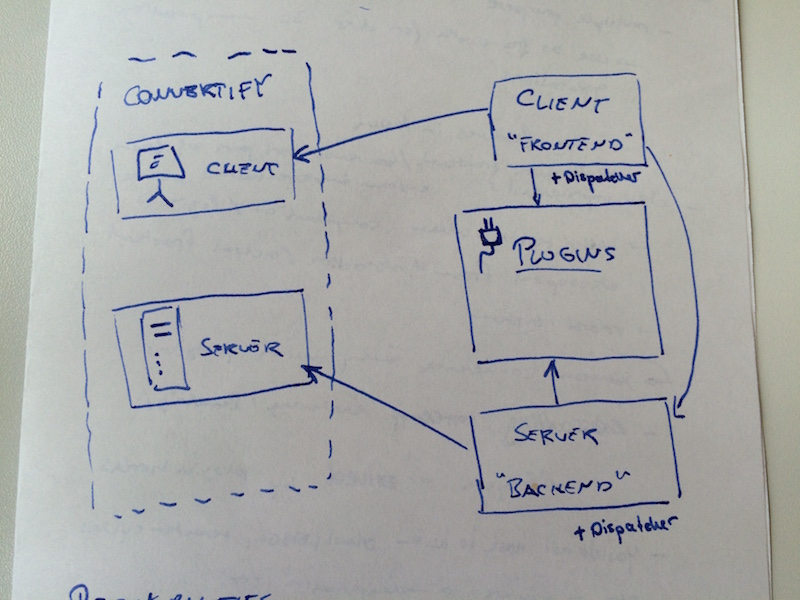
\includegraphics[width=1\columnwidth]{Images/03-architecture_overview_current.JPG}
\caption{Main Packages of the Platener Architecture}
\label{fig:architectureOverviewCurrent}
\end{figure}

Platener is designed to enabled web-based manipulation and rendering of {\threedmodel}s. Figure \ref{fig:architectureOverviewCurrent} shows the major packages \emph{Convertify}, \emph{Client}, \emph{Server} and \emph{Plugins}. The arrows indicate dependencies between the packages. The architecture emphasizes a uni-directional data and event flow. Similar to mobile application design, lifecycle events and the concept of delegation\footnote{\url{https://developer.apple.com/library/ios/documentation/General/Conceptual/DevPedia-CocoaCore/Delegation.html}} establish clear communication among packages. 

% begin block comment
\iffalse
\begin{itemize}
\item platener built on top of...
\item 4 major packages: convertify, client, server and plugins
\item optimized towards: working with 3d-models in webgl environment
\item plugin-based: allow interchangeable computation logic/ conversion methods
\item combination of lifecycle-based communication and explicit calls via dispatchers (related work: mobile application design, mediator pattern)
\item explicit communication between packages
\end{itemize}
\fi
% end block comment

\subsection{Package Responsibilities}

Each package takes over a set of distinct responsibilities ensuring decoupled components. Thus a flexible, maintainable system is created.

\emph{Convertify} provides generic tools which support plugins in manipulating {\threedmodel}s. This includes utilities for vector analysis as well as rendering routines and scene management. The application lifecycle can be initiated and observed via a \emph{Bundle}. A Bundle represents an instance of the application's computation unit. The Client and Server packages run a Bundle.

The \emph{Client} package gives the look and feel of the application. Where Convertify can be reused as-is for many different purposes, the Client package has to be rewritten from scratch. This package contains frontend components. The developer can choose any template engine\footnote{\url{http://www.sitepoint.com/overview-javascript-templating-engines/}} which serves the application's purpose. So the Client actually wires up the {\userinterface} and the computation logic.

The \emph{Server} package is the headless counterpart to the Client package. A Command Line Interface enables the user to run the application without a browser. The Server also satisfies requests from the Client, such as caching and loading models in a RESTful interaction\footnote{\url{http://www.drdobbs.com/web-development/restful-web-services-a-tutorial/240169069}}. Again, the Server package has to be rewritten for a custom application.

\emph{Plugins} provide an exchangeable set of features which are used by the Client and Server package. A Plugin interacts with the Scene and its {\threedmodel}s via lifecycle events. E.g. a concrete conversion strategy provided by Platener is implemented by a single Plugin. Plugin features can be enabled for Client, Server or both. 

% block comment
\iffalse
\begin{itemize}
\item convertify: generic tools, helpers for 3d rendering, scene management, model manipulation, platener independent
\item client: look and feel, ux user interactions, wiring up/ firing up computations, implemented for platener
\item server: model storage/ cache, REST interaction, headless version of client, CLI-tool chain, implemented for platener
\item plugins: conversion specific computation and logic units, addons for frontend and backend, platener independent
\end{itemize}
\fi
% end block comment

\subsection{Motivation}
\begin{itemize}
\item multpiple purpose:
\item use as framework for other 3D manipulation applications (related work: mechanism mining, etc)
\item web service --> highly available, cross platform
\item plug features in and out
\item because concrete frontend/ backend not part of framework, custom implementations possible (no vendor lock)

\item dev improvements:
\item better testing of computation/ logic because decoupled from ux
\item robust system
\item --> loose coupling of plugins, high cohesion in plugins
\item --> isolated testing/ development possible
\item solve cross-cuts: rendering/ loading <> lifecycle of plugins (eventbased)
\item you do not have to know about WEBGL, render cycles etc. to provide a 3D manipulation tool
\item --> minimize web-domain knowledge as CG-devs are often unfamiliar with this environment
\end{itemize}

\subsection{Discussion "vs Brickify"}

\begin{figure}
\label{fig:architecture_overview_brickify}
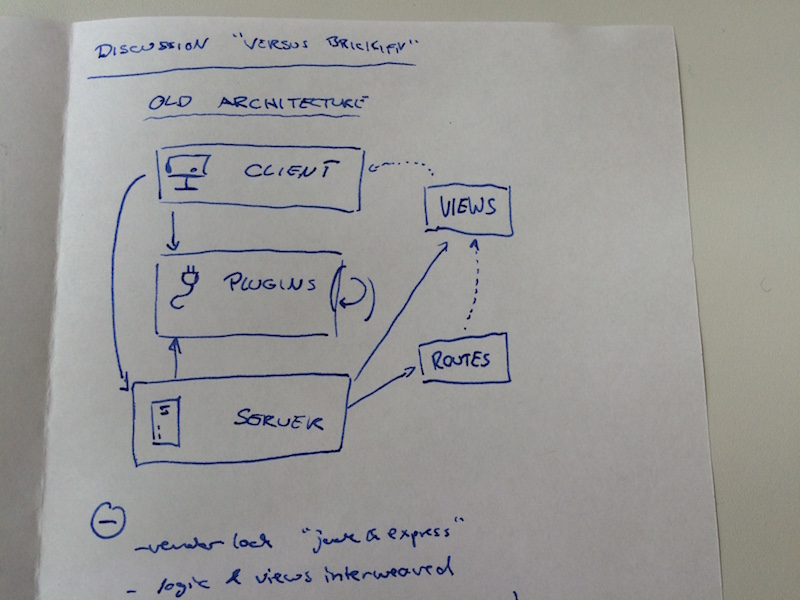
\includegraphics[width=1\columnwidth]{Images/03-architecture_overview_brickify.JPG}
\caption{Main Packages of the former Brickify Architecture}
\end{figure}

\textbf{pros}
\begin{itemize}
\item fast enhancements as only views/ routes have to be adapted
\item less interfacing because frontend <> logic tightly coupled
\end{itemize}

\textbf{cons} 
\begin{itemize}
\item vendor lock: jade and express
\item logic and views interweaved: high coupling --> hard testing, hard maintainability, hard to change things
\item implicit plugin communication 
\item complex management of custom 3d manipulation tools would require a lot of rewrites because of view/ logic mix
\end{itemize}




\section{Convertify Package and its Plugin Architecture}


\subsection{Convertify Purpose - Application Helpers}

\begin{itemize}
\item entry points
\item headless startup
\item basic logic for 3dmodel manipulation (import, meshconversion)
\item scenegraph and rendering (nodes, refs for syncobjects in brickify)
\item plugin interaction (hooks)
\item application helpers (threeHelper, renderHelper, commons (we should move commons to convertify))
\end{itemize}

\subsection{Platener's Plugins}

%The Client package provides the look and feel of Platener. The Server package manages communication between frontend and data storage.

The plugins composed into Platener provides its computations logic and WebgGL scene rendering. We will give a brief introduction of each plugin in the following paragraphs.

\subsubsection{Coordinate System}

This plugin provides orientation enhancements for the WebGL scene. Rendering xyz-axes and a an axis-aligned grid, users can grasp alignment and dimensions of {\threedmodel}s. Figure \ref{fig:architecture_overview_coordinate_system} shows the coordinate system in the WebGL view.

\begin{figure}
\label{fig:architecture_overview_coordinate_system}
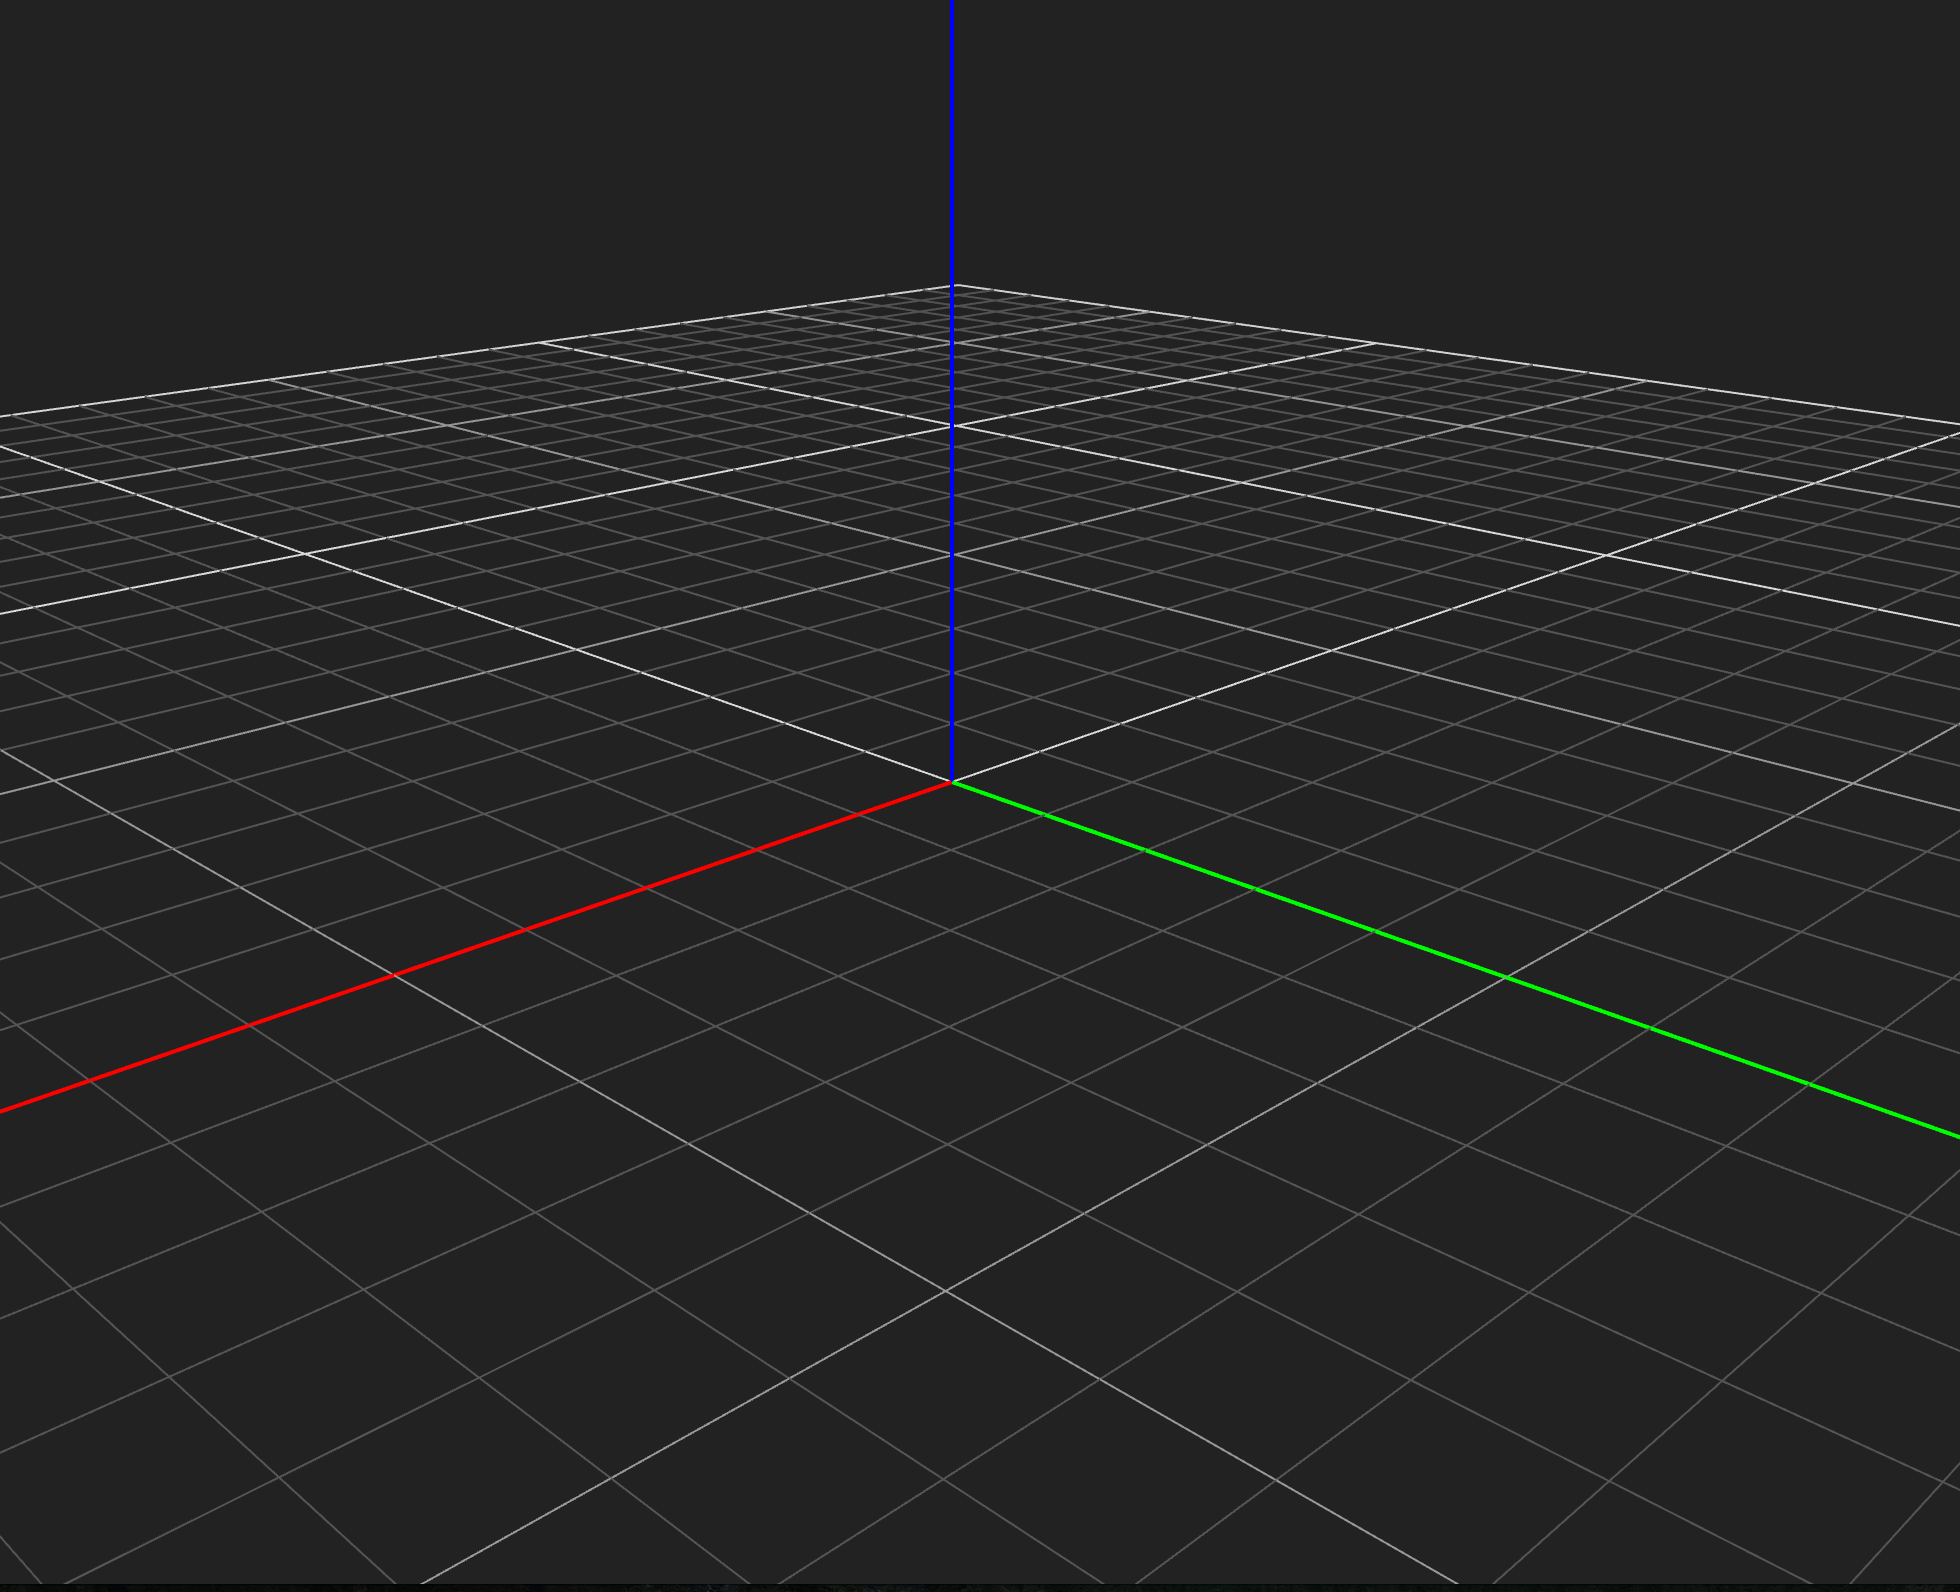
\includegraphics[width=1\columnwidth]{Images/03-architecture_overview_coordinate_system.png}
\caption{An empty scene showing the coordinate system.}
\end{figure}

\subsubsection{Platener Pipeline}

The Platener Pipeline plugin is the main computation unit. The plugin defines multiple {\fabmethod}s. A {\fabmethod} is a conversion approach of a \threedmodel. Multiple components, which can manipulate the input model, are chained after another to produce 2D- or 3D-output. For example construction plans for the original input model as {\svgfile}s. 

\subsubsection{Node Visualizer}

We visualize the results of the Platener Pipeline plugin in the WebGL view. The Node Visualizer plugin renders the results of each component of each {\fabmethod} respectively.

\subsubsection{Scoring}

When multiple {\fabmethod}s are run, we want to choose the best fitted conversion as output. Thus each {\fabmethod} is scored by a method-specific scoring algorithm. This plugin provides these scoring algorithms.

\subsubsection{Solution Selection}

This plugin utilizes the Platener Pipeline plugin and the Scoring plugin to run and evaluate all {\fabmethod}s. It outputs the result of the {\fabmethod} with the best score and notifies the Dispatcher.

\subsubsection{Isolated Testing}

While we worked at different stages of a linearly executed {\fabmethod} in parallel, we needed a mechanism to test each component of the {\fabmethod} before its preceeding or succeeding components were finished. The Isolated Testing plugin provides an isolated environment, which allows to execute a single component of a {\fabmethod} with pre-defined input.

%- working in parallel, while needing inputs of work in progress
%- validate & visualize test scenarios for separate pipeline steps (components of a \fabmethod)
%- provide input for a given step and compute/ render results for just that step

\subsection{Control Flow via Dispatchers}

As Platener is composed of multiple plugins, which either represent computation logic or render components, we have to know exactly when each of these plugins will interact with the system. We propose a Dispatcher component, behaving similar to the mediator pattern\footnote{\url{https://sourcemaking.com/design_patterns/mediator}}.

\subsubsection{Dispatcher}

The Dispatcher organizes the communication between plugins and client, plugins and server and plugins and plugins in a single place. 

\myNotes{TODO: diagrams}

\subsubsection{Control Flow}

\begin{itemize}
\item wiring up plugins
\item explictely calling plugin hooks
\end{itemize}

\subsubsection{vs Brickify only plugin hooks}

\begin{itemize}
\item ++ pros
\item loading sequence control (impossible to repair)
\item explicit execution behavior
\item ... (look at notes on desk)
\item 
\item -- cons
\item boilerplate code
\end{itemize}

\subsection{Platener Pipeline}


\begin{enumerate}
\item Overview/ Purpose/ Plugin Structure

\item \begin{itemize}
\item conversion strategies & logic
\end{itemize}

\item Pipeline Steps

What are pipeline steps?
Where to be found in the code?
How are they used in Platener Pipeline?

\item Fabrication Methods


\begin{enumerate}
\item Plate Method


\item Stacked Plates Method


\item Classifier Method

\end{enumerate}

\item Immutable Pipeline State


\begin{enumerate}
\item Overview/ Purpose


\item Immutability


\item Implementation Details

\end{enumerate}
\end{enumerate}

\subsection{Node Visualizer}


\begin{enumerate}
\item Overview - Visual Debugging


\item Visualizer and Visualizations


\item Interwoven with Platener Pipeline


\begin{enumerate}
\item Role of Immutability


\item Extracting Intermediate Data of the Pipeline

\end{enumerate}
\end{enumerate}

\subsection{Isolated Testing}


\begin{enumerate}
\item Static Input and Expected Output


\item Testables

\end{enumerate}

\subsection{Scorer and Solution Selection}


Selecting the best estimated solution by default.

\section{Client Package}


\subsection{Overview - Custom Frontend Code}


\subsection{React Templates}


\subsection{Redux Data-driven Control Flow}


\begin{enumerate}
\item Dispatcher and Redux `dispatch`

\end{enumerate}

\section{Server Package}


\subsection{Overview - Custom Server Code}


\subsection{Model Cache}


\subsection{Test Pipeline}


\begin{enumerate}
\item Headless Conversion of Objects


\item Reports


\item Benchmarks

\end{enumerate}

\end{document}